\chapter{An introduction to Treewidth} \label{ch:treewidth}

The concept of tree decomposition and treewidth was first introduced by Robertson and Seymour to prove the famous graph minor theorem, which we state here for reference. 

% TODO: check if the statement is correct.
\begin{theorem}[Graph Minor Theorem, Robertson and Seymour \cite{robertson_seymour_1}]
	For any infinite sequence of graphs $G_1, G_2, \ldots$, there exist indices $i < j$ such that $G_i$ is a minor of $G_j$.
\end{theorem}

Treewidth later was proved to be very useful in many different areas of graph theory. 
As core algorithmic idea in this dissertation relies on treewidth, it is worth our effort to introduce treewidth and its properties in detail.

\section{Treewidth and its Elemetary Properties}

\begin{definition}[Tree Decomposition]
	Let $G$ be a finite graph and $V$ its vertex set. A \define{tree decomposition} of $G$ is a pair $(T, \{X_t\}_{t \in V(T)})$ where $T$ is a tree and $\{X_t\}_{t \in V(T)}$ is a family of subsets of $V$ (called bags) such that
	\begin{enumerate}
		\item $\bigcup_{t \in V(T)} X_t = V$,
		\item If vertices $u, v \in G$ are adjacent, there exists a $t \in T$  such that $u, v \in X_t$.
		\item Let $a, b$ be vertices of $T$. Since $T$ is a tree, there is a unique path connecting $a$ and $b$, which is denoted as $P$. If $v \in G$ and $v \in X_a, v \in X_b$, then for all $c \in P$, we have $v \in X_c$.
	\end{enumerate}

	Let $X_t$ be the bag such that $ \forall i \in T, |X_t| \geq |X_i|$ (That is, $X_t$ is the bag of the largest order). The \define{width} of the tree decomposition $(T, \{X_t\})$ is $|X_t| - 1$.
\end{definition}

\begin{definition}[Treewidth]
	The \define{tree width} of a graph $G$ is the minimum width over all of its tree decompositions.
\end{definition}

Tree decomposition requires the existence of a bag that contains all the adjacent vertices. 
If $u,v \in G$ and $\exists t$ such that $ u, v \in X_t $, however, it does not guarantee that $u$ and $v$ are adjacent in $G$.

\begin{example}[All graphs have a trivial tree decomposition]
	Let $G$ be a graph with vertex set $V$. Then $(T, \{X_t\})$ is a tree decomposition of $G$ where $T$ is a single node and $X_t = V$. The width of this tree decomposition is $|V| - 1$.

	Therefore, the treewidth of any graph $G$ is bounded above by $|V| - 1$.
	By Zorn's lemma, there must exist a tree decomposition of $G$ with minimum width.
\end{example}

Let us look at some examples of tree decomposition.

\begin{example}[Tree decomposition of a Tree]
	Let $G$ be a tree. We can construct a tree decomposition of $G$ in the following way.
	\begin{enumerate}
		\item Let each vertex of $G$ be a bag that contains only itself.
		\item On each edge of $G$, add a bag that contains the two endpoints of the edge.
	\end{enumerate}
	An example of this tree decomposition is shown in figure \ref{fig:tree_decomposition_of_tree}. 
	This gives the treewidth of a tree is $1$. 
	For any tree with at least one edge, there must be a bag that contains two or more vertices. This proves that the treewidth of a non-trivial tree is exactly $1$.
\end{example}

\begin{figure}[ht]
	\centering
	% Graph Board TikZ export
% Exported: 2026-08-10T20:25:43.207Z
% Title: Untitled Graph
% Nodes: 19, Edges: 15

\begingroup
% --- Colors (define-if-not-already-defined) ---
\providecolor{zxRed}{RGB}{232,165,165}   % X spiders
\providecolor{zxGreen}{RGB}{216,248,216} % Z spiders
\providecolor{zxYellow}{RGB}{255,255,0}     % hadamard 

\tikzset{
    EMPTY/.style={minimum size=3.4mm,
        outer sep=-1.7mm},
    DOT/.style={inner sep=0mm, minimum size=3.4mm, shape=circle,
        draw=black, outer sep=-0.5mm, line width=1pt},
    BLACK_DOT/.style={minimum size=2mm, inner sep=0.3mm,
        outer sep=-0.15mm, fill=black, shape=circle},
    WORD_BALL/.style={draw=black, shape=rectangle, minimum size=6.5mm,
        rounded corners=3.2mm, inner sep=1.2mm, outer sep=-1.0mm,
        scale=1, font={\large\boldmath}, line width=1pt},
    GREEN_DOT/.style={DOT, fill=zxGreen},
    GREEN_WORD_BALL/.style={WORD_BALL, fill=zxGreen},
    RED_DOT/.style={DOT, fill=zxRed},
    RED_WORD_BALL/.style={GREEN_WORD_BALL, fill=zxRed},
    YELLOW_BOX/.style={fill=zxYellow, draw=black, line width=1pt, shape=rectangle, inner sep=0.6mm,
        minimum height=3.4mm, minimum width=3.4mm,
        font={\large\boldmath}},
    EDGE/.style={draw=black, line width=1pt},
    BLUE_DASHED_EDGE/.style={EDGE, draw=blue, dashed}
}
\pgfdeclarelayer{edgelayer}
\pgfdeclarelayer{nodelayer}
\pgfsetlayers{edgelayer,nodelayer,main}

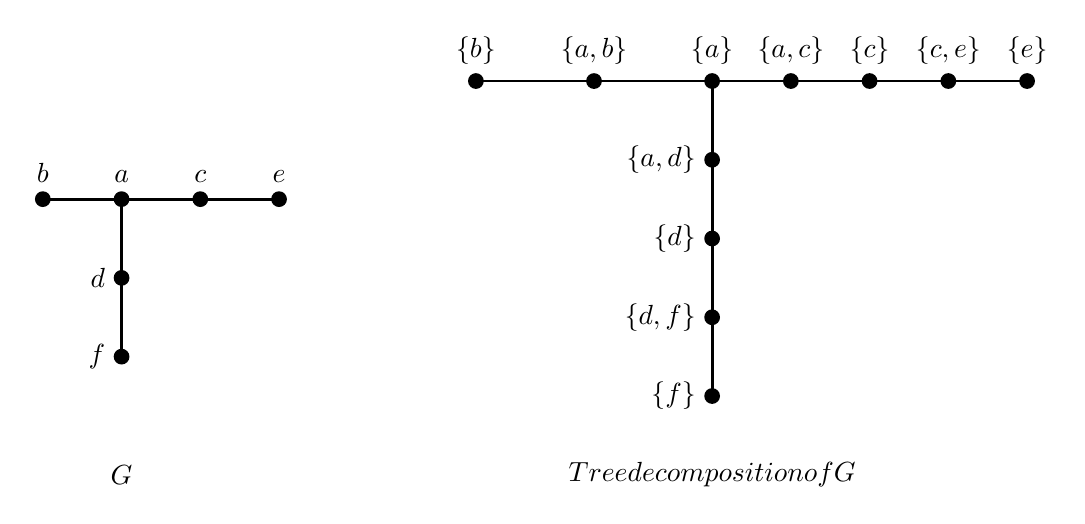
\begin{tikzpicture}
    \begin{pgfonlayer}{nodelayer}
        \node [label=above:{$a$}, BLACK_DOT] (1) at (-5.13158, 0.18421) {};
        \node [label=left:{$f$}, BLACK_DOT] (2) at (-5.13158, -1.81579) {};
        \node [label=above:{$b$}, BLACK_DOT] (3) at (-6.13158, 0.18421) {};
        \node [label=left:{$d$}, BLACK_DOT] (4) at (-5.13158, -0.81579) {};
        \node [label=above:{$c$}, BLACK_DOT] (5) at (-4.13158, 0.18421) {};
        \node [label=above:{$e$}, BLACK_DOT] (6) at (-3.13158, 0.18421) {};
        \node [EMPTY] (7) at (-5.13158, -3.31579) {$G$};
        \node [label=above:{$\{a\}$}, BLACK_DOT] (8) at (2.36842, 1.68421) {};
        \node [label=left:{$\{d\}$}, BLACK_DOT] (9) at (2.36842, -0.31579) {};
        \node [label=above:{$\{a,b\}$}, BLACK_DOT] (10) at (0.86842, 1.68421) {};
        \node [label=left:{$\{a,d\}$}, BLACK_DOT] (11) at (2.36842, 0.68421) {};
        \node [label=above:{$\{a, c\}$}, BLACK_DOT] (12) at (3.36842, 1.68421) {};
        \node [label=above:{$\{c\}$}, BLACK_DOT] (13) at (4.36842, 1.68421) {};
        \node [label=above:{$\{b\}$}, BLACK_DOT] (14) at (-0.63158, 1.68421) {};
        \node [label=left:{$\{d, f\}$}, BLACK_DOT] (15) at (2.36842, -1.31579) {};
        \node [label=left:{$\{f\}$}, BLACK_DOT] (16) at (2.36842, -2.31579) {};
        \node [label=above:{$\{c,e\}$}, BLACK_DOT] (17) at (5.36842, 1.68421) {};
        \node [label=above:{$\{e\}$}, BLACK_DOT] (18) at (6.36842, 1.68421) {};
        \node [EMPTY] (19) at (2.36842, -3.31579) {$\text{Tree decomposition of } G$};
    \end{pgfonlayer}
    \begin{pgfonlayer}{edgelayer}
        \draw[EDGE] (3) to (1);
        \draw[EDGE] (4) to (1);
        \draw[EDGE] (5) to (1);
        \draw[EDGE] (2) to (4);
        \draw[EDGE] (6) to (5);
        \draw[EDGE] (10) to (8);
        \draw[EDGE] (11) to (8);
        \draw[EDGE] (12) to (8);
        \draw[EDGE] (9) to (11);
        \draw[EDGE] (13) to (12);
        \draw[EDGE] (14) to (10);
        \draw[EDGE] (16) to (15);
        \draw[EDGE] (9) to (15);
        \draw[EDGE] (18) to (17);
        \draw[EDGE] (17) to (13);
    \end{pgfonlayer}
\end{tikzpicture}

\endgroup
	\caption{A tree decomposition of a tree.}
	\label{fig:tree_decomposition_of_tree}
\end{figure}

\begin{example}[Tree Decomposition of Some Random Graphs]
	See figure \ref{fig:tree_decomposition_of_random_graph} for an example of a tree decomposition of a triangulated graph.
\end{example}

\begin{figure}[ht]
	\centering
	% Graph Board TikZ export
% Exported: 2026-08-10T21:07:29.267Z
% Title: Untitled Graph
% Nodes: 15, Edges: 15

\begingroup
% --- Colors (define-if-not-already-defined) ---
\providecolor{zxRed}{RGB}{232,165,165}   % X spiders
\providecolor{zxGreen}{RGB}{216,248,216} % Z spiders
\providecolor{zxYellow}{RGB}{255,255,0}     % hadamard 

\tikzset{
    EMPTY/.style={minimum size=3.4mm,
        outer sep=-1.7mm},
    DOT/.style={inner sep=0mm, minimum size=3.4mm, shape=circle,
        draw=black, outer sep=-0.5mm, line width=1pt},
    BLACK_DOT/.style={minimum size=2mm, inner sep=0.3mm,
        outer sep=-0.15mm, fill=black, shape=circle},
    WORD_BALL/.style={draw=black, shape=rectangle, minimum size=6.5mm,
        rounded corners=3.2mm, inner sep=1.2mm, outer sep=-1.0mm,
        scale=1, font={\large\boldmath}, line width=1pt},
    GREEN_DOT/.style={DOT, fill=zxGreen},
    GREEN_WORD_BALL/.style={WORD_BALL, fill=zxGreen},
    RED_DOT/.style={DOT, fill=zxRed},
    RED_WORD_BALL/.style={GREEN_WORD_BALL, fill=zxRed},
    YELLOW_BOX/.style={fill=zxYellow, draw=black, line width=1pt, shape=rectangle, inner sep=0.6mm,
        minimum height=3.4mm, minimum width=3.4mm,
        font={\large\boldmath}},
    EDGE/.style={draw=black, line width=1pt},
    BLUE_DASHED_EDGE/.style={EDGE, draw=blue, dashed}
}
\pgfdeclarelayer{edgelayer}
\pgfdeclarelayer{nodelayer}
\pgfsetlayers{edgelayer,nodelayer,main}

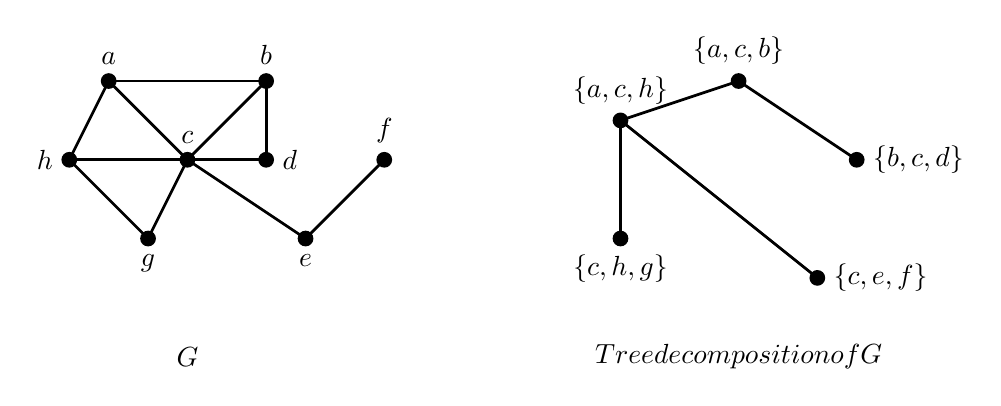
\begin{tikzpicture}
    \begin{pgfonlayer}{nodelayer}
        \node [EMPTY] (1) at (-2.96667, -2.1) {$G$};
        \node [EMPTY] (2) at (4.03333, -2.1) {$\text{Tree decomposition of } G$};
        \node [label=above:{$a$}, BLACK_DOT] (3) at (-3.96667, 1.4) {};
        \node [label=left:{$h$}, BLACK_DOT] (4) at (-4.46667, 0.4) {};
        \node [label=below:{$g$}, BLACK_DOT] (5) at (-3.46667, -0.6) {};
        \node [label=below:{$e$}, BLACK_DOT] (6) at (-1.46667, -0.6) {};
        \node [label=above:{$f$}, BLACK_DOT] (7) at (-0.46667, 0.4) {};
        \node [label=above:{$b$}, BLACK_DOT] (8) at (-1.96667, 1.4) {};
        \node [label=right:{$d$}, BLACK_DOT] (9) at (-1.96667, 0.4) {};
        \node [label=above:{$c$}, BLACK_DOT] (10) at (-2.96667, 0.4) {};
        \node [label=below:{$\{c,h, g\}$}, BLACK_DOT] (11) at (2.53333, -0.6) {};
        \node [label=above:{$\{a,c,h\}$}, BLACK_DOT] (12) at (2.53333, 0.9) {};
        \node [label=above:{$\{a,c,b\}$}, BLACK_DOT] (13) at (4.03333, 1.4) {};
        \node [label=right:{$\{b, c, d\}$}, BLACK_DOT] (14) at (5.53333, 0.4) {};
        \node [label=right:{$\{c,e,f\}$}, BLACK_DOT] (15) at (5.03333, -1.1) {};
    \end{pgfonlayer}
    \begin{pgfonlayer}{edgelayer}
        \draw[EDGE] (3) to (10);
        \draw[EDGE] (4) to (10);
        \draw[EDGE] (3) to (4);
        \draw[EDGE] (5) to (10);
        \draw[EDGE] (4) to (5);
        \draw[EDGE] (3) to (8);
        \draw[EDGE] (10) to (8);
        \draw[EDGE] (8) to (9);
        \draw[EDGE] (6) to (7);
        \draw[EDGE] (10) to (9);
        \draw[EDGE] (10) to (6);
        \draw[EDGE] (11) to (12);
        \draw[EDGE] (13) to (12);
        \draw[EDGE] (13) to (14);
        \draw[EDGE] (15) to (12);
    \end{pgfonlayer}
\end{tikzpicture}

\endgroup

	\caption{A tree decomposition of a triangulated graph.}
	\label{fig:tree_decomposition_of_random_graph}
\end{figure}

The following lemma will be useful.

\begin{lemma}
	Let $G$ be a graph and $T$ its tree decomposition of at least three vertices. Let $a \in T$.
	If deleting $a$ from $T$ produces at least two subgraphs of $T$, which we label as $C_1, C_2$, that are disconnected, then the subgraph of $G$ induced by the vertices in $\bigcup_{t\in C_1} \{X_t\} - A $ and $\bigcup_{t\in C_2} \{X_t\} - A $ are disconnected.
\end{lemma} \label{lem:tree_decomposition_disconnected_subgraph}

\begin{proof}
	It is sufficient to show that for all $v\in G_1$ and $u \in G_2$, $v$ is not adjacent to $u$. 

	Assume that $v \in G_1$ and $u \in G_2$ and they are adjacent. 
	Let $v \in X_s$, $u \in X_r$, and let $P_0$ be the unique path from $s$ to $r$ in $T$. By our assumption, $P_0$ contains the point $a$.

	By property 2 of tree decomposition, there exists $t \in T$ such that $v, u \in X_t$.
	Since $T$ is connected, there exists a path $P_1$ from $s$ to $t$ and path $P_2$ from $r$ to $t$.
	If none of them pass through $a$, then there is a cycle in $T$ consisting of $P_0$, $P_1$, and $P_2$. This contradicts the fact that $T$ is a tree. Therefore, at least one of them must pass through $a$.

	Without loss of any generality, let $P_1$ pass through $a$.
	By property 3 of tree decomposition, $P_1$ is a path whose endpoints are bags that contain $v$, so by property 3 again the bag $X_a$ contains $v$ as well.
	This is a contradiction to the assumption that $v \in G_1$. (Recall that $G_1$ does not contain any vertices that are in $X_a$)
\end{proof}

\begin{example}[Treewidth of a Complete Graph]
	The treewidth of a complete graph $K_n$ is $n-1$, as all tree decompositions of $K_n$ must contain a bag that contains all vertices of $K_n$.

	To prove this claim, assume $T$ is a tree decomposition of $K_n$ and let $X_i$ be the largest bag of $T$ that does not contain all vertices of $K_n$. 
	Since $X_i$ does not contain all vertices of $K_n$, there exists a vertex $v \in K_n$ such that $v \notin X_i$, which is in the bag $X_j$ for some $j$. Again, as $v$ is connected to all other vertices and $X_j$ does not contain all vertices, there must be a third bag in $T$. 

	In a tree with at least three vertices, there must exist a vertex $a$ such that deleting $a$ from $T$ will produce at least two disconnected subgraphs of $T$.
	Now we can invoke lemma \ref{lem:tree_decomposition_disconnected_subgraph} , which states that deleting $a$ from $T$ will produce at least two disconnected subgraphs of $T$. This is not possible as $K_n$ is a complete graph, so all vertices are connected. 

	Therefore, all tree decompositions of $K_n$ must contain a bag that contains all vertices of $K_n$, which proves the claim.
\end{example}

If graph $G$ is a minor of $H$, then the treewidth of $G$ is less than or equal to the treewidth of $H$.
The definition of graph minor is presented here for reference.

\begin{definition}[Graph Minor]
	Let $G$ and $H$ be two graphs. We say that $G$ is a \define{minor} of $H$ if $G$ can be obtained from $H$ by a sequence of the following operations:
	\begin{enumerate}
		\item Deleting an edge,
		\item Deleting a vertex,
		\item Contracting an edge.
	\end{enumerate}
	The process of contracting an edge $e = (u, v)$ is to delete the edge $e$ and merge the two vertices $u$ and $v$ into a single vertex $w$. The new vertex $w$ is adjacent to all the neighbors of $u$ and $v$.
\end{definition}

\begin{lemma}[Graph Minor and Treewidth]\label{lem:minor_treewidth}
	Let $G$ and $H$ be two graphs. If $G$ is a minor of $H$, then the treewidth of $G$ is less than or equal to the treewidth of $H$.
\end{lemma}

The proof of this lemma is presented in section \ref{sec:proofs}.

We can use lemma \ref{lem:minor_treewidth} to prove various lower bounds on the treewidth. 

\begin{corollary}\label{cor:treewidth_delta_lower_bound}
	Let $\delta$ be the minimum vertex degree of a graph $G$. The treewidth of $G$ is at least $\delta$.
\end{corollary}

\begin{proof}
	We can continuously contract edges in $G$ until we obtain a complete graph $K_{\delta + 1}$. By lemma \ref{lem:minor_treewidth}, the treewidth of $G$ is at least the treewidth of $K_{\delta + 1}$, which is $\delta$.
\end{proof}

Using these lemmas, we can find the treewidth of more complicated graphs.

\begin{example}
	The treewidth of a circle graph is $2$.
	By corollary \ref{cor:treewidth_delta_lower_bound}, the treewidth of a circle graph is at least $2$ as the minimum vertex degree of a circle graph is $2$.
	We can construct a tree decomposition of a circle graph with width $2$ as follows.

	Let vertex $a$ be the start of the cycle. Delete one edge next to $a$ and treat the rest of the graph as a tree, with the maximum bag of size $2$.
	Adding $a$ to all bags of the tree decomposition gives a tree decomposition of the circle graph with bags of maximum size $3$ and width $2$.

	See figure \ref{fig:tree_decomposition_of_circle_graph} for an example.
\end{example}

\begin{figure}[ht]
	\centering
	% Graph Board TikZ export
% Exported: 2026-08-11T21:10:27.536Z
% Title: Untitled Graph
% Nodes: 12, Edges: 11

\begingroup
% --- Colors (define-if-not-already-defined) ---
\providecolor{zxRed}{RGB}{232,165,165}   % X spiders
\providecolor{zxGreen}{RGB}{216,248,216} % Z spiders
\providecolor{zxYellow}{RGB}{255,255,0}     % hadamard 
\providecolor{zxBlue}{RGB}{68,126,255}     % hadamard 


\tikzset{
    EMPTY/.style={minimum size=3.4mm,
        outer sep=-1.7mm},
    DOT/.style={inner sep=0mm, minimum size=3.4mm, shape=circle,
        draw=black, outer sep=-0.5mm, line width=1pt},
    BLACK_DOT/.style={minimum size=2mm, inner sep=0.3mm,
        outer sep=-0.15mm, fill=black, shape=circle},
    WORD_BALL/.style={draw=black, shape=rectangle, minimum size=6.5mm,
        rounded corners=3.2mm, inner sep=1.2mm, outer sep=-1.0mm,
        scale=1, font={\large\boldmath}, line width=1pt},
    GREEN_DOT/.style={DOT, fill=zxGreen},
    GREEN_WORD_BALL/.style={WORD_BALL, fill=zxGreen},
    RED_DOT/.style={DOT, fill=zxRed},
    RED_WORD_BALL/.style={GREEN_WORD_BALL, fill=zxRed},
    YELLOW_BOX/.style={fill=zxYellow, draw=black, line width=1pt, shape=rectangle, inner sep=0.6mm,
        minimum height=3.4mm, minimum width=3.4mm,
        font={\large\boldmath}},
    EDGE/.style={draw=black, line width=1pt},
    BLUE_DASHED_EDGE/.style={-, dashed, dash pattern=on 2pt off 0.5pt, ultra thick, zxBlue}
}
\pgfdeclarelayer{edgelayer}
\pgfdeclarelayer{nodelayer}
\pgfsetlayers{edgelayer,nodelayer,main}

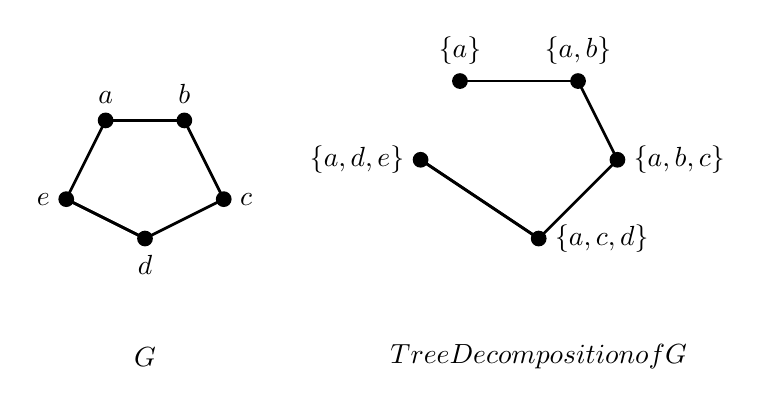
\begin{tikzpicture}
    \begin{pgfonlayer}{nodelayer}
        \node [label=above:{$b$}, BLACK_DOT] (1) at (-1.91667, 0.91667) {};
        \node [label=above:{$a$}, BLACK_DOT] (2) at (-2.91667, 0.91667) {};
        \node [label=left:{$e$}, BLACK_DOT] (3) at (-3.41667, -0.08333) {};
        \node [label=below:{$d$}, BLACK_DOT] (4) at (-2.41667, -0.58333) {};
        \node [label=right:{$c$}, BLACK_DOT] (5) at (-1.41667, -0.08333) {};
        \node [label=right:{$\{a, b, c\}$}, BLACK_DOT] (6) at (3.58333, 0.41667) {};
        \node [label=above:{$\{a, b\}$}, BLACK_DOT] (7) at (3.08333, 1.41667) {};
        \node [label=left:{$\{a, d, e\}$}, BLACK_DOT] (8) at (1.08333, 0.41667) {};
        \node [label=right:{$\{a, c, d\}$}, BLACK_DOT] (9) at (2.58333, -0.58333) {};
        \node [label=above:{$\{a\}$}, BLACK_DOT] (10) at (1.58333, 1.41667) {};
        \node [EMPTY] (11) at (-2.41667, -2.08333) {$G$};
        \node [EMPTY] (12) at (2.58333, -2.08333) {$\text{Tree Decomposition of }G$};
    \end{pgfonlayer}
    \begin{pgfonlayer}{edgelayer}
        \draw[EDGE] (1) to (2);
        \draw[EDGE] (2) to (3);
        \draw[EDGE] (3) to (4);
        \draw[EDGE] (1) to (5);
        \draw[EDGE] (5) to (4);
        \draw[EDGE] (6) to (7);
        \draw[EDGE] (6) to (9);
        \draw[EDGE] (9) to (8);
        \draw[EDGE] (4) to (3);
        \draw[EDGE] (8) to (9);
        \draw[EDGE] (10) to (7);
    \end{pgfonlayer}
\end{tikzpicture}

\endgroup
	\caption{A tree decomposition of a circle graph.}
	\label{fig:tree_decomposition_of_circle_graph}
\end{figure}


\section{Treewidth and Tensor Contraction.}

It is possible to derive an upper bound for tensor contraction cost using treewidth

\begin{theorem}[Treewidth Bound on Tensor Contraction Cost]\label{thm:treewidth_tensor_contraction} 
	Let $G$ be a tensor network with no lose bonds and regarded as a graph. 
	Let all the bonds of $G$ be dimension $d$.
	It is possible to contract $G$ with a cost of $O(d^{\text{tw}(G*) + 1})$, where $\text{tw}(G*)$ is the treewidth of the line graph of $G$.
\end{theorem}

Markov and Shi first discovered this connection \cite{Markov_2008}.
The theorem is constructive, and there exists an algorithm that to find such a contraction order, which we break down in the following steps.

\begin{definition}[Line Graph]
	Let $G$ be a graph. The \define{line graph} of $G$, denoted as $G^*$, is a graph such that each vertex of $G^*$ represents an edge of $G$, and two vertices of $G^*$ are adjacent if and only if their corresponding edges share a common endpoint in $G$.
\end{definition}

\begin{example}
	See figure \ref{fig:line_graph_1} for an example of a graph with 6 vertices and 7 edges and its line graph with 7 vertices and 11 edges.
\end{example}

\begin{figure}[ht]
	\centering
	% Graph Board TikZ export
% Exported: 2026-08-13T21:30:02.255Z
% Title: Untitled Graph
% Nodes: 22, Edges: 17

\begingroup
% --- Colors (define-if-not-already-defined) ---
\providecolor{zxRed}{RGB}{232,165,165}   % X spiders
\providecolor{zxGreen}{RGB}{216,248,216} % Z spiders
\providecolor{zxYellow}{RGB}{255,255,0}     % hadamard 
\providecolor{zxBlue}{RGB}{68,126,255}     % hadamard 


\tikzset{
    EMPTY/.style={minimum size=3.4mm,
        outer sep=-1.7mm},
    DOT/.style={inner sep=0mm, minimum size=3.4mm, shape=circle,
        draw=black, outer sep=-0.5mm, line width=1pt},
    BLACK_DOT/.style={minimum size=2mm, inner sep=0.3mm,
        outer sep=-0.15mm, fill=black, shape=circle},
    WORD_BALL/.style={draw=black, shape=rectangle, minimum size=6.5mm,
        rounded corners=3.2mm, inner sep=1.2mm, outer sep=-1.0mm,
        scale=1, font={\large\boldmath}, line width=1pt},
    GREEN_DOT/.style={DOT, fill=zxGreen},
    GREEN_WORD_BALL/.style={WORD_BALL, fill=zxGreen},
    RED_DOT/.style={DOT, fill=zxRed},
    RED_WORD_BALL/.style={GREEN_WORD_BALL, fill=zxRed},
    YELLOW_BOX/.style={fill=zxYellow, draw=black, line width=1pt, shape=rectangle, inner sep=0.6mm,
        minimum height=3.4mm, minimum width=3.4mm,
        font={\large\boldmath}},
    EDGE/.style={draw=black, line width=1pt},
    BLUE_DASHED_EDGE/.style={-, dashed, dash pattern=on 2pt off 0.5pt, ultra thick, zxBlue},
    GRAY_DASHED_EDGE/.style={-, dashed, dash pattern=on 3pt off 1.5pt, thick, lightgray}
}
\pgfdeclarelayer{edgelayer}
\pgfdeclarelayer{nodelayer}
\pgfsetlayers{edgelayer,nodelayer,main}

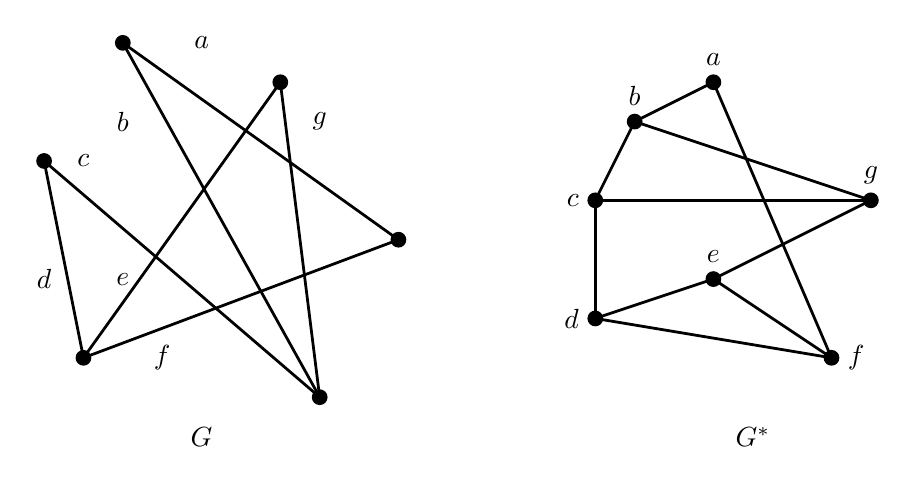
\begin{tikzpicture}
    \begin{pgfonlayer}{nodelayer}
        \node [BLACK_DOT] (1) at (-3.18182, 2.38636) {};
        \node [BLACK_DOT] (2) at (0.31818, -0.11364) {};
        \node [BLACK_DOT] (3) at (-4.18182, 0.88636) {};
        \node [BLACK_DOT] (4) at (-3.68182, -1.61364) {};
        \node [BLACK_DOT] (5) at (-1.18182, 1.88636) {};
        \node [BLACK_DOT] (6) at (-0.68182, -2.11364) {};
        \node [EMPTY] (7) at (-2.18182, -2.61364) {$G$};
        \node [EMPTY] (8) at (4.81818, -2.61364) {$G^*$};
        \node [label=above:{$a$}, BLACK_DOT] (9) at (4.31818, 1.88636) {};
        \node [label=above:{$b$}, BLACK_DOT] (10) at (3.31818, 1.38636) {};
        \node [label=left:{$c$}, BLACK_DOT] (11) at (2.81818, 0.38636) {};
        \node [label=left:{$d$}, BLACK_DOT] (12) at (2.81818, -1.11364) {};
        \node [label=above:{$e$}, BLACK_DOT] (13) at (4.31818, -0.61364) {};
        \node [label=above:{$g$}, BLACK_DOT] (14) at (6.31818, 0.38636) {};
        \node [label=right:{$f$}, BLACK_DOT] (15) at (5.81818, -1.61364) {};
        \node [EMPTY] (16) at (-2.18182, 2.38636) {$a$};
        \node [EMPTY] (17) at (-3.18182, 1.38636) {$b$};
        \node [EMPTY] (18) at (-3.68182, 0.88636) {$c$};
        \node [EMPTY] (19) at (-4.18182, -0.61364) {$d$};
        \node [EMPTY] (20) at (-3.18182, -0.61364) {$e$};
        \node [EMPTY] (21) at (-2.68182, -1.61364) {$f$};
        \node [EMPTY] (22) at (-0.68182, 1.38636) {$g$};
    \end{pgfonlayer}
    \begin{pgfonlayer}{edgelayer}
        \draw[EDGE] (4) to (3);
        \draw[EDGE] (6) to (3);
        \draw[EDGE] (4) to (5);
        \draw[EDGE] (6) to (5);
        \draw[EDGE] (4) to (2);
        \draw[EDGE] (2) to (1);
        \draw[EDGE] (1) to (6);
        \draw[EDGE] (9) to (10);
        \draw[EDGE] (9) to (15);
        \draw[EDGE] (10) to (11);
        \draw[EDGE] (10) to (14);
        \draw[EDGE] (11) to (12);
        \draw[EDGE] (11) to (14);
        \draw[EDGE] (12) to (13);
        \draw[EDGE] (12) to (15);
        \draw[EDGE] (13) to (15);
        \draw[EDGE] (13) to (14);
    \end{pgfonlayer}
\end{tikzpicture}

\endgroup
	\caption{Graph $G$ and its line graph $G^*$. The edges of $G$ and vertices of $G^*$ are labeled with the same alphabet.}
	\label{fig:line_graph_1}
\end{figure}


\section{Miscellaneous Proofs}\label{sec:proofs}

\begin{proof}[Proof of Lemma \ref{lem:minor_treewidth}]
	We only need to prove that if a graph $G$ can be obtained from $H$ by performing one of the three operations, then the treewidth of $G$ is less than or equal to the treewidth of $H$. The lemma follows as any minor can be obtained by a finite sequence of these three operations.

	Let $T$ be a tree decomposition of $H$.
	We have three cases to consider.
	\begin{enumerate}
		\item If $G$ is obtained from $H$ by deleting an edge, then $T$ is also a tree decomposition of $G$. 
		\item If $G$ is obtained from $H$ by deleting a vertex $v$, let $T'$ be the tree decomposition of $G$ isomorphic to $T$ with $v$ removed from all bags. (We allow empty bags). It is clear that $T'$ is a tree decomposition of $G$ and the width of $T'$ is less than or equal to the width of $T$.
		\item If $G$ is obtained from $H$ by contracting an edge $(u, v)$. Let $w$ denote the new vertex after contraction. 
		Let $T'$ be the tree decomposition of $G$ isomorphic to $T$ with $u$ and $v$ replaced by a new vertex $w$ in all bags that contain $u$ or $v$. 
	\end{enumerate}

	In all cases, we can construct a tree decomposition of $G$ from a tree decomposition of $H$ with width less than or equal to the width of $T$. Therefore, the treewidth of $G$ is less than or equal to the treewidth of $H$.
\end{proof}


